\section{Preliminary Results}

\subsection{PhaseNet Overview}

PhaseNet is a neural network designed to correct distortions and restore the phase of a received signal. It is particularly useful for applications involving \textbf{phase modulation} or \textbf{Phase Shift Keying (PSK)}. However, the model encounters challenges when calculating the phase error between the \textbf{estimated} and \textbf{real values}, especially when the angles reside in different quadrants of the complex plane. This issue arises because the error is calculated as the angular difference, and transitions between quadrants (e.g., second to third) can cause significant increases in error.

\textbf{Key Problem:} Angle values are typically represented in the range \(-\pi\) to \(\pi\) (in libraries like PyTorch and NumPy), which complicates accurate error measurement when phase wrapping occurs.

\subsection*{Solution}
To address this issue, the following method was adopted:
\begin{enumerate}
    \item \textbf{Fixed Radius Assumption:} Instead of working with the full complex number, the ground truth is normalized to a \textbf{radius of 1}. The focus is solely on the \textbf{phase (angle)}. Using Euler's formula, the complex number is represented as:
    \[
    O(\hat{\theta}) = e^{i\hat{\theta}} = \cos(\hat{\theta}) + i \cdot \sin(\hat{\theta}),
    \]
    where \(\hat{\theta}\) is the estimated phase.

    \item \textbf{Mean Squared Error (MSE) for Real and Imaginary Parts:}  
    The error is measured in the rectangular form by calculating the MSE for the real and imaginary components separately:
    \[
    MSE(\hat{\theta}) = \frac{1}{2} \left( E \left[ (\cos(\hat{\theta}) - x_{\text{real}})^2 \right] + E \left[ (\sin(\hat{\theta}) - x_{\text{imag}})^2 \right] \right),
    \]
    where \(x_{\text{real}}\) and \(x_{\text{imag}}\) are the real and imaginary parts of the ground truth, respectively.
\end{enumerate}

\begin{figure}[H]
    \centering
    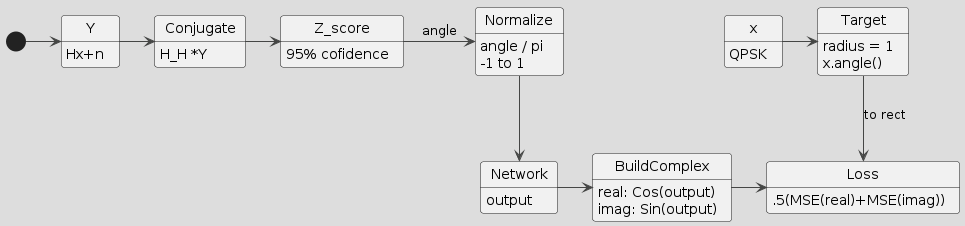
\includegraphics[width=0.8\textwidth]{Figures/PhasNet.png} 
    \caption{Proccessing stages}
    \label{fig:example}
\end{figure}

\subsection*{Preprocessing Stages}
The preprocessing of the input signal plays a \textbf{critical role} in enabling the network to converge effectively. The key steps are:
\begin{enumerate}
    \item Multiply the received signal \(Y\) by the \textbf{Hermitian transpose} of the channel \(H^H\) to obtain \(H^H Y\) as the input.
    \item Apply a \textbf{Z-score filter} to eliminate outliers, ensuring that 95\% of the values fall within a confidence interval.
    \item Normalize angles: Convert the angle values from the range \([- \pi, \pi]\) to the range \([-1, 1]\).
\end{enumerate}

\subsection{Network Parameters}
PhaseNet is implemented using a \textbf{PyTorch \texttt{nn.Sequential}} block with the following layers:

\begin{table}[H]
    \centering
    \caption{PhaseNet Network Parameters}
    \label{tab:phasenet_parameters}
    \begin{tabular}{l l l}
        \toprule
        \textbf{Layer}             & \textbf{Output Shape}      & \textbf{Number of Parameters} \\
        \midrule
        \texttt{nn.Linear(48, 240)} & (batch\_size, 240)         & \( (48 + 1) \times 240 = 11,760 \) \\
        \texttt{nn.Hardtanh()}      & (batch\_size, 240)         & 0                             \\
        \texttt{nn.Linear(240, 720)} & (batch\_size, 720)        & \( 2 \times 240^2 + 2 \times 240 = 346,320 \) \\
        \texttt{nn.Linear(720, 240)} & (batch\_size, 240)        & \( 4 \times 240^2 + 2 \times 240 = 1,388,160 \) \\
        \texttt{nn.Hardtanh()}      & (batch\_size, 240)         & 0                             \\
        \texttt{nn.Linear(240, 48)} & (batch\_size, 48)          & \( (240 + 1) \times 48 = 11,568 \) \\
        \bottomrule
    \end{tabular}
\end{table}

\subsection{Hyperparameters}
The following hyperparameters are used for PhaseNet:
\begin{table}[H]
    \centering
    \caption{PhaseNet Hyperparameters}
    \label{tab:phasenet_hyperparameters}
    \begin{tabular}{l l}
        \toprule
        \textbf{Hyperparameter}    & \textbf{Value}       \\
        \midrule
        Batch Size                 & 10                  \\
        QAM Order                  & 16                  \\
        Number of Epochs           & 2                   \\
        Learning Rate              & \( 8 \times 10^{-5} \) \\
        Input Size                 & 48                  \\
        Hidden Size                & 240                 \\
        SNR (Signal-to-Noise Ratio) & 35 dB               \\
        \bottomrule
    \end{tabular}
\end{table}

\noindent The total number of parameters in PhaseNet is approximately 1,757,808, which corresponds to around 13.39 MB of memory usage.


\subsection{BER vs SNR Analysis}

The graph compares the \textbf{Bit Error Rate (BER)} performance of two techniques, \textbf{LMMSE} (Linear Minimum Mean Square Error) and \textbf{PhaseNet}, as a function of the \textbf{Signal-to-Noise Ratio (SNR)} for QPSK modulation.

\begin{figure}[H]
    \centering
    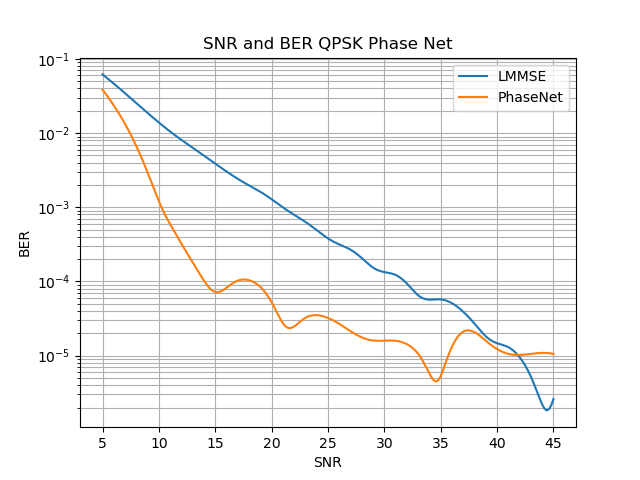
\includegraphics[width=0.8\textwidth]{Figures/QPSKvsLMMSEPhasNet.png}
    \caption{BER performance between PhaseNet and LMSE}
    \label{fig:example_image}
\end{figure}

\begin{enumerate}
    \item \textbf{Overall Behavior:}
    \begin{itemize}
        \item Both techniques show a decreasing BER as the SNR increases, which is expected because higher SNR improves signal clarity.
        \item PhaseNet consistently achieves a lower BER than LMMSE across the entire SNR range.
    \end{itemize}
    
    \item \textbf{Low SNR (5--15 dB):}
    \begin{itemize}
        \item In this range, both PhaseNet and LMMSE exhibit significant BER values.
        \item However, PhaseNet achieves an improvement over LMMSE, with the BER for PhaseNet decreasing faster as the SNR increases.
    \end{itemize}
    
    \item \textbf{Mid SNR (15--30 dB):}
    \begin{itemize}
        \item PhaseNet continues to outperform LMMSE, maintaining a lower BER.
        \item LMMSE shows a reduction in BER, but the performance gap between the two techniques widens slightly as the SNR increases.
    \end{itemize}
    
    \item \textbf{High SNR (30--45 dB):}
    \begin{itemize}
        \item Both techniques achieve very low BER values at high SNR.
        \item PhaseNet achieves the lowest BER, particularly around \textbf{35--40 dB}, where LMMSE still exhibits slightly higher error rates.
        \item At \textbf{45 dB}, LMMSE shows a small spike in BER, while PhaseNet remains relatively stable.
    \end{itemize}
\end{enumerate}